\documentclass[tikz,border=2pt]{standalone}
\usetikzlibrary{arrows.meta,automata,positioning}
\usepackage{siunitx}
\definecolor{celadon}{rgb}{0.67, 0.88, 0.69}
\definecolor{lightskyblue}{rgb}{0.61, 0.87, 1.0}
\definecolor{bluebell}{rgb}{0.64, 0.64, 0.82}

\begin{document}
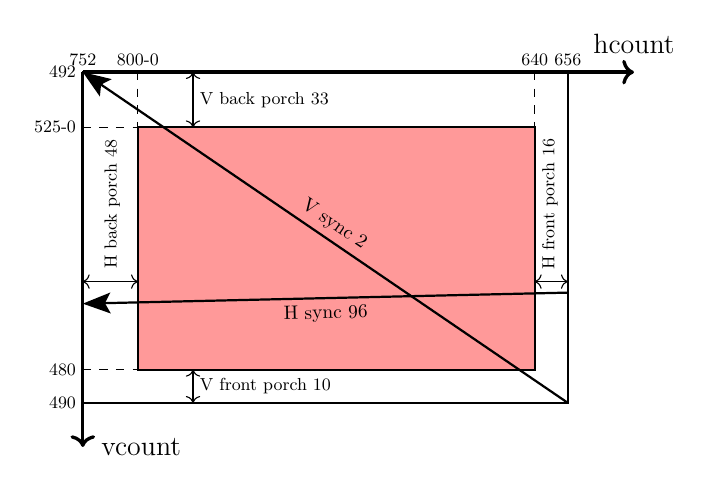
\begin{tikzpicture}[scale=0.7, transform shape]
% =====================
% ASSI
% =====================
\draw[very thick,->] (0,0) -- (10,0) node[above=0.2cm]{\Large hcount};
\draw[very thick,->] (0,0) -- (0,-6.8) node[right=0.2cm]{\Large vcount};
\draw[thick] (0,0) rectangle (8.8,-6);

% =====================
% AREA ATTIVA
% =====================
\fill[red!40]
(1,-1) rectangle (8.2,-5.4);
\draw[thick]
(1,-1) rectangle (8.2,-5.4);

% =====================
% LINEE DI RIFERIMENTO
% =====================
\draw[dashed] (1,0) -- (1,-1);
\draw[dashed] (0,-1) -- (1,-1);
\draw[dashed] (0,-5.4) -- (1,-5.4);
\draw[dashed] (8.2,0) -- (8.2,-1);

% =====================
% DIAGONALI SYNC
% =====================
\draw[thick, arrows = {-Stealth[length=10pt, inset=2pt]}] (8.8,-6) -- (0,0)
node[midway,sloped,above]{V sync 2};
\draw[thick, arrows = {-Stealth[length=10pt, inset=2pt]}] (8.8,-4) -- (0,-4.2)
node[midway,sloped,below]{H sync 96};

% =====================
% QUOTE ORIZZONTALI
% =====================
\draw[<->] (0,-3.8) -- (1,-3.8)
node[pos=0.8,above=1.4cm,rotate=90]{\small H back porch 48};
\draw[<->] (8.2,-3.8) -- (8.8,-3.8)
node[pos=0.9,above=1.4cm,rotate=90]{\small H front porch 16};

% =====================
% QUOTE VERTICALI
% =====================
\draw[<->] (2,0) -- (2,-1)
node[midway,right]{\small V back porch 33};
\draw[<->] (2,-5.4) -- (2,-6)
node[midway,right]{\small V front porch 10};

% =====================
% NUMERI SUGLI ASSI
% =====================
\node[above] at (1,0) {\small 800-0};
\node[above] at (8.2,0) {\small 640};
\node[above] at (8.8,0) {\small 656};
\node[above] at (0,0) {\small 752};
\node[left] at (0,-1) {\small 525-0};
\node[left] at (0,-5.4) {\small 480};
\node[left] at (0,-6) {\small 490};
\node[left] at (0,0) {\small 492};

\end{tikzpicture}
\end{document}